% ********** Rozdział 4 **********
\chapter{Harmonogram realizacji projektu}

\label{sec:harmon_proj}
\section{Diagram Gantta}

\begin{figure}[H]
    \begin{center}
	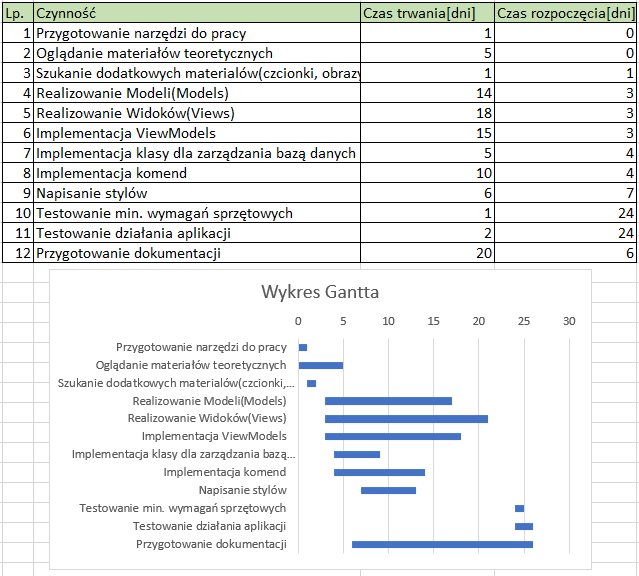
\includegraphics[height=10cm]{images/Wykres_Gantta.png}
        \caption{Wykres Gantta}
    \end{center}
\end{figure}

Zacząłem pracę nad projektem z przygotowania narzędzi do pracy(ustawienia Visual Studio) i oglądania materiałów teoretycznych. Bardzo mi pomogły serie filmików na temat "Architektura MVVM w WPF" na YouTube({\color{blue}\href{https://youtu.be/fZxZswmC_BY?si=Fs_RE23INJFVoy1r}{link}}). Następnie próbowałem zrobić swoją aplikacje na bazie otrzymanej teorii. 

W końcu pozostało mi przetestować minimalne wymagania sprzętowe za pomocą wirtualnej maszyny.


\section{Repozytorium}
Do kontroli wersji oraz przechowywania wykorzystałem systemu Git oraz serwisu internetowego GitHub. Wszystkie pliki źródłowe projektu oraz dokumentacji są umieszczone w tym linku - {\color{blue}\href{https://github.com/clowd1e/Szpital}{Repozytorium GitHub}}.

% ********** Koniec rozdziału **********